\chapter{Introduzione}
\section{ Premessa }

\textbf{Def - Sistemi dinamici:}  sono un'evoluzione temporale di un ingresso e un'uscita, vengono modellati dalle \textbf{equazioni differenziali}.\\
Vedremo sono funzioni monodimensionali (cioè dipendenti solo dal tempo) ma in realtà possiamo benissimo avere più dimensioni.\\
I modelli ci danno una stima del comportamento di una sistema, in particolare il modello delle equazioni differenziali si può svolgere: nel tempo, nel dominio della trasformata di Laplace (utile con i segnali esponenziali e sinusoidali) e nel dominio della trasformata di Fourier (è un restrizione di Laplace, è utile nei segnali sinusoidali).\\
Studieremo le proprietà dei sistemi, di queste la più importante è la stabilità.\\
\textbf{Modelliamo un sistema} come fosse una scatola nera, avrà un segnale come input e output (es. suono 1D, immagine 2D).\\
I sistemi ci servono per vari motivi: possono facilitare la trasmissione di un segnale, migliorarlo accentuando alcune informazioni o eliminandone altre (filtraggio).\\
Vogliamo vedere i sistemi come \textbf{funzioni matematiche} (pag. 69 libro "Structure and Interpretation of Signals and Systems")\\

\begin{figure}
	\centering
	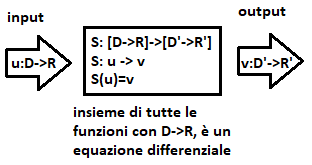
\includegraphics[width=0.7\linewidth]{immagini/sistema}
	\caption{ modello di un sistema come scatola nera}
	\label{fig:sistema}
\end{figure}



$ \forall s \in D' $ allora $ v(s)=(S(u))(s)\in R'  $ \\

\pagebreak

Abbiamo tre tipi di sistemi:\\
- Continui: operano su segnali continui\\
- Discreti: operano su segnali discreti\\
- Ibridi fra continui e discreti (non li vedremo)\\

\begin{figure}[h]
	\centering
	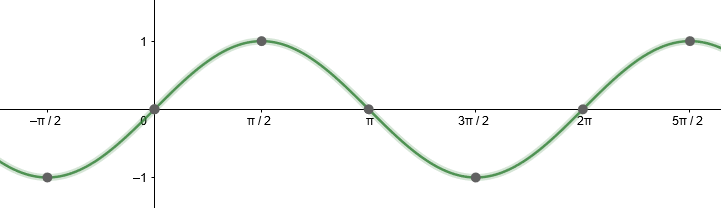
\includegraphics[width=0.7\linewidth]{immagini/seno}
	\caption{Segnale continuo}
	\label{fig:seno}
\end{figure}


\begin{figure}[h]
	\centering
	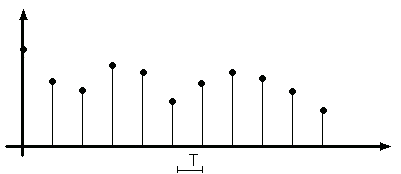
\includegraphics[width=0.7\linewidth]{immagini/tempo_discreto}
	\caption{ Segnale discreto}
	\label{fig:tempodiscreto}
\end{figure}

\textbf{Quantizzazione e campionamento}\\
Per andare da analogico a digitale (A->D) ho bisogno di campionamento e quantizzazione.\\

Campionamento: trasformiamo il dominio. Non ho sempre perdita di dati.\\

\begin{figure}[h]
	\centering
	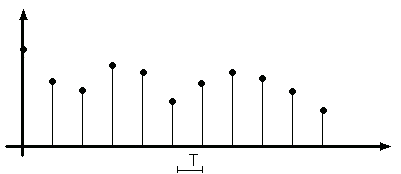
\includegraphics[width=0.7\linewidth]{immagini/tempo_discreto}
	\caption{ Segnale campionato nel tempo}
	\label{fig:tempodiscreto}
\end{figure}

\pagebreak
Quantizzazione: trasformiamo il codominio. Ha sempre perdita di informazione.\\

\begin{figure}[h]
	\centering
	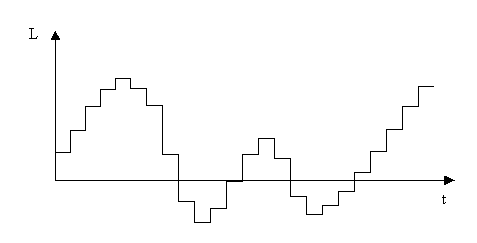
\includegraphics[width=0.7\linewidth]{immagini/quantizzato}
	\caption{ Segnale sinusoidale quantizzato nelle ampiezze}
	\label{fig:quantizzato}
\end{figure}

\textbf{Sistemi LTI}\\
Studiamo un tipo particolare di sistemi, che hanno due proprietà: linearità e tempo invarianza (L=lineari, TI=tempo invarianti).\\
- Linearità:\\
Se $ v_{1}=S(u_{1}) $ e $ v_{2}=S(u_{2})  $ 
allora $ S(\alpha u_{1} + \beta u_{2}) 
= \alpha S(u_{1}) + \beta S(u_{2})
= \alpha v_{1} + \beta v_{2} $ con $ \alpha , \beta \in C^{*} $ \\
Oppure grazie al \textbf{principio di sovrapposizione degli effetti} ( stabilisce che per un sistema dinamico lineare l'effetto di una somma di perturbazioni in ingresso è uguale alla somma degli effetti prodotti da ogni singola perturbazione): \\
$ S( \sum_{i=0}^n \alpha_i u_i ) 
=  \sum_{i=0}^n \alpha_i S( u_i )
$ \\
La linearità è dovuta alle equazioni differenziali, all'interno hanno la derivata prima che è essa stessa lineare.\\
- Tempo invariante:\\
 Significa che l'uscita non dipende esplicitamente dal tempo, cioè se un ingresso x(t) produce l'uscita y(t) allora per ogni ingresso traslato $x(t+ \delta )$ si ha un'uscita traslata dello stesso fattore $y(t+ \delta )$.\\
 
 $u(t+ t_0 ) \rightarrow v(t+ t_0 )$
 
\begin{figure}[h]
	\centering
	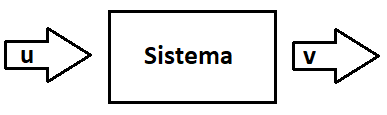
\includegraphics[width=0.7\linewidth]{immagini/sistema2}
	\caption{ Sistema generico }
	\label{fig:sistema2}
\end{figure}

\begin{figure}[h]
	\centering
	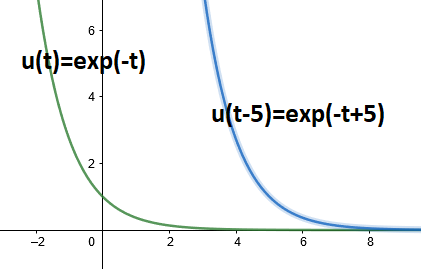
\includegraphics[width=0.7\linewidth]{immagini/esponenziale}
	\caption{ Esempio di tempo invariante }
	\label{fig:esponenziale}
\end{figure}

\pagebreak

I sistemi LTI che studieremo sono definiti da equazioni differenziali a coefficienti costanti.

Per i sistemi continui useremo il modello:
\begin{equation*}
\sum\limits_{i=0}^n a_{i} \frac{ d^{i} v }{ dt^{i}  } = \sum\limits_{i=0}^m b_{i} \frac{ d^{i} u }{ dt^{i}  }
\tag{1}\label{equation 1}
\end{equation*}
con $u$ e $v$ funzioni con dominio uguale a $\mathbb{R}$. In generale abbiamo $n\geq m$.


Per i sistemi discreti useremo il modello:
\begin{equation*}
\sum\limits_{i=0}^n a_{i} v(k-i) = \sum\limits_{i=0}^m b_{i} u(k-i)
\end{equation*}
con $u$ e $v$ funzioni con dominio uguale a $\mathbb{Z}$ e $ k \in \mathbb{Z} $.

\subsection*{Sistemi SISO}
Per semplicità considereremo solo i sistemi SISO, cioè single input single output. Ma in generale i sistemi sono MIMO, cioè multiple input multiple output (questi non li vedremo).

\subsection*{Esempio semplice di un sistema}

Nel dominio del tempo rappresentiamo un sistema $S$ continuo come: \\
\begin{equation*}
S: [\mathbb{R} \rightarrow \mathbb{R}] \rightarrow [\mathbb{R} \rightarrow \mathbb{R}]
\end{equation*}

Abbiamo anche visto che modelliamo i sistemi con le derivate (che ehhh non ci piacciono molto) e vorremmo quindi qualcosa di più semplice. Usiamo Laplace (salvatore del popolo) che trasforma le derivate in moltiplicazioni ("Trasformò acqua in vino" semicit.). Le moltiplicazioni sono semplici e belle (insomma tanto love per le moltiplicazioni e per Laplace $\heartsuit$).\\

Nel dominio complesso o delle frequenze rappresentiamo quindi il sistema $S$ continuo come: \\
\begin{equation*}
S: [\mathbb{C} \rightarrow \mathbb{C}] \rightarrow [\mathbb{C} \rightarrow \mathbb{C}]
\end{equation*}

\begin{figure}[h]
	\centering
	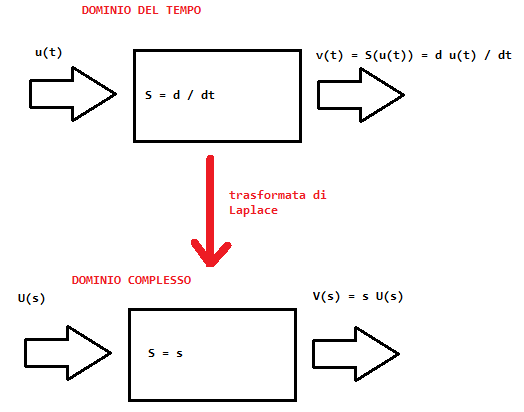
\includegraphics[width=0.7\linewidth]{immagini/LaplaceLove}
	\caption{ Come Laplace trasforma dal dominio del tempo a quello complesso }
	\label{fig: Sistema Laplace}
\end{figure}

\subsection*{Esempio di sistema discreto}
Consideriamo il sistema: \\
\begin{equation*}
	\begin{split}
	S: [\mathbb{Z} \rightarrow \mathbb{R}] \rightarrow [\mathbb{Z} \rightarrow \mathbb{R}] \\
	u \mapsto S(u) = v
	\end{split}
\end{equation*}
dove $v(n) = \dfrac{u(n)+u(n-1)}{2} \in \mathbb{R} $. Cioè l'output è $\forall n $ la media dell'input attuale e dell'input precedente (sistema moving average).\\
$u(n)$ può essere una qualsiasi funzione discreta. Prendiamo due esempi diversi di input.\\


Per primo esempio prendo come input:
\begin{equation*}
u(n)=
\begin{cases} 
	1, & \mbox{se }n\geq 0 \\ 
	0, & \mbox{altrimenti}
\end{cases} 
\end{equation*}

\begin{figure}[h]
	\centering
	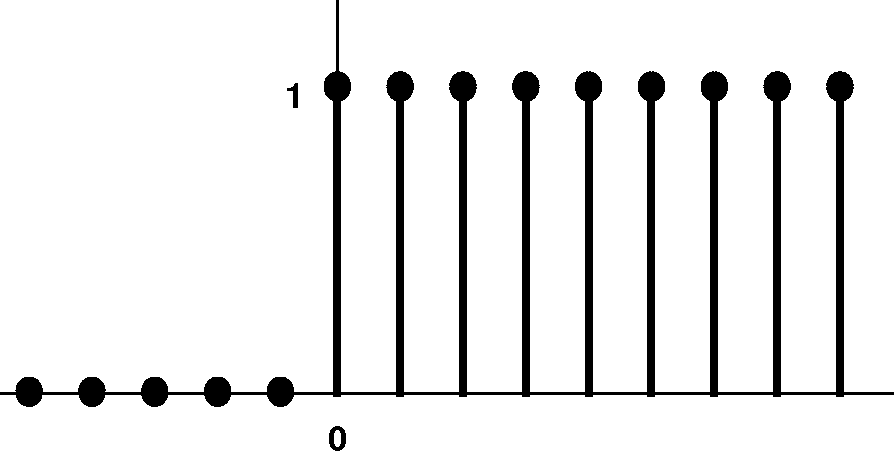
\includegraphics[scale=0.5]{immagini/gradino}
	\caption{ La funzione gradino (unit step) come input }
	\label{fig: Unit step}
\end{figure}

\pagebreak

Avrò come output:
\begin{equation*}
v(n)=
\begin{cases} 
0, & \mbox{se }n < 0 \\ 
1/2, & \mbox{se }n = 0 \\ 
1, & \mbox{se }n > 0
\end{cases} 
\end{equation*}

\begin{figure}[h]
	\centering
	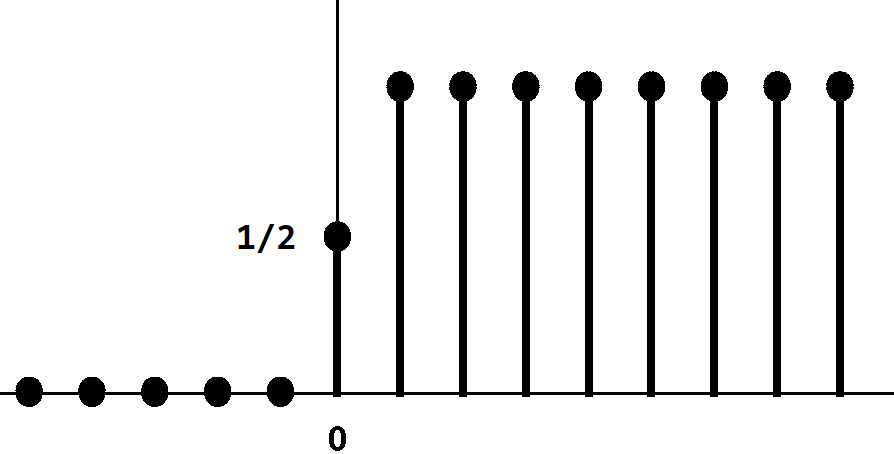
\includegraphics[scale=0.5]{immagini/gradinoMedia}
	\caption{ L'output del sistema moving average con in input la funzione gradino}
	\label{fig: Output sistema moving average gradino}
\end{figure}
Per secondo esempio prendo come input:
\begin{equation*}
u(n)= \cos(2\pi f n)
\end{equation*}
dove $n \in \mathbb{Z} $ e $f \in \mathbb{R}_{+}^{*}$\\
Avrò come output:
\begin{equation*}
v(n)= S(u)(n) = \frac{1}{2} (\cos(2\pi f n) + \cos(2\pi f (n-1))) = R\cos( 2\pi f n + \theta) \in \mathbb{R}^{*}
\end{equation*}
dove $\theta = \frac{1}{2} \arctan(\frac{ \sin (-2\pi f)    }{1+\cos(2\pi f)})$ e $ R = \sqrt{ 2+2\cos(2\pi f)} \in \mathbb{R}^{*}$\\
NB: Amplifico l'input sinudoidale con R ma il periodo e la frequenza rimangono invariate. In output quindi avrò ancora un segnale sinusoidale (questo fenomeno lo studieremo nella frequence responce).

\pagebreak

\section{ Ripasso sui numeri complessi }

\subsection*{Rappresentazione cartesiana di un numero complesso}
Definiamo $s$ un numero complesso, $ s = x+jy$ con $j=\sqrt{-1}$ o $j^{2} = -1$.\\
$x$ è la parte reale di $s$ e viene scritta come $Re(s)$ \\
$y$ è la parte immaginaria di $s$ e viene scritta come $Im(s)$.\\
Un numero viene definito \textbf{ immaginario puro} se ha $ Re(s) = 0 $ e $ Im(s) = y $, cioè ha la parte reale nulla.

\subsection*{Il piano complesso}

\begin{figure}[h]
	\centering
	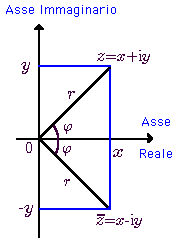
\includegraphics[scale=1.2]{immagini/pianoComplesso}
	\caption{ Piano complesso }
	\label{fig: piano complesso}
\end{figure}

\subsection*{Il coniugato complesso}
Il coniugato complesso di $s$ è $ \bar{s} = x -jy $.\\
Da notare come $s\bar{s} = (x+jy)(x-jy) = x^{2}+y^{2}$.\\

\subsection*{L'insieme dei numeri complessi}
$\mathbb{C} =$ \{ $s / s = x+jy, x,y \in \mathbb{R} $\} 

\subsection*{Rappresentazione polare di un numero complesso}

$s$ si può scrivere anche in forma:
\begin{equation*}
 s = \rho (cos\theta + j sen\theta)
\end{equation*}
con $\theta \in \mathbb{R}$ .\\
Definiamo rho come il raggio di $s$, cioè: \\
$\rho := |s| = \sqrt{x^{2}+y^{2}} = \sqrt{ Re^{2}(s)+Im^{2}(s)} = \sqrt{s\bar{s}} = |\bar{s}|$.\\
Definiamo theta come "l'angolo" di $s$, cioè è l'argomento di $s$: \\
$ \theta = Arg(s)$ \\
OSS: $\theta$ non è univoco, devo imporre un limite, che può essere:
$\theta = [0,2\pi)$ oppure $\theta = (-\pi, \pi] $ \\
Da notare come: $Arg(s) = Arg(\bar{s})$


\subsection*{Operazioni con i numeri complessi}
Consideriamo due numeri complessi $ s_{0} = x_{0}+jy_{0} $ e $ s_{1} = x_{1}+jy_{1} $ \\

\textbf{Somma:} \\
$ s_{0} + s_{1} = ( x_{0}+x_{1} ) + j (y_{0} + y_{1}) $ \\

\textbf{Prodotto:} \\
$ s_{0} s_{1} = ( x_{0} + j y_{0})( x_{1} + j y_{1}) $ \\
$ = x_{0} x_{1} - y_{0} y_{1} + j (x_{0} y_{1} + x_{1} y_{0} ) $ questa purtroppo non ci è molto utile.\\
Proviamo quindi ad usare la rappresentazione polare, troviamo che: \\
$ = \rho_{0} (cos\theta_{0} + j sin\theta_{0})\rho_{1} (cos\theta_{1} + j sin\theta_{1}) $ \\
$ = \rho_{0} \rho_{1} ( \cos\theta_{0} \cos\theta_{1} + j \cos\theta_{0} \sin\theta_{1} + j \sin\theta_{0} \cos\theta_{1}-\sin\theta_{0} \sin\theta_{1}) $ \\
$ = \rho_{0} \rho_{1} ( \cos (\theta_{0} + \theta_{1}) + j \sin ( \theta_{0} + \theta_{1} )) $ \\
L'ultima riga è molto più facile da ricordare e da utilizzare.
NB: Dobbiamo sempre rimanere con $\theta \in (-\pi , \pi]$

\begin{figure}[h]
	\centering
	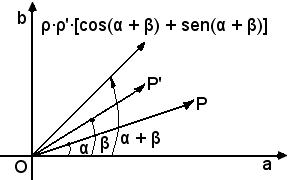
\includegraphics[scale=0.5]{immagini/moltiplicazioneComplessi}
	\caption{ Moltiplicazione fra due complessi }
	\label{fig: Moltiplicazione fra due complessi}
\end{figure}

NB: $ |s_{0} s_{1}| = |s_{0}||s_{1}|$ \\
$ Arg( s_{0} s_{1} ) = Arg(s_{0} ) + Arg( s_{1} )$ sempre $ \in (-\pi , \pi]$\\
$ \bar{s_{0} s_{1}} = \bar{s_{0} } \bar{s_{1}}$ \\

\textbf{Inverso:} \\
Se $ s \neq 0 $ dove $ 0 = 0 + j0 $,\\
definiamo l'inverso di un complesso come $ \frac{ \bar{s} }{ |s|^{2}} = \frac{x-jy}{x^{2} + y^{2}} $ \\
\begin{proof}[Dim]
	\begin{equation*}
	\begin{split}
	s \frac{1}{s} = s \frac{ \bar{s} }{s \bar{s}} = 1 \\
	\end{split}
	\end{equation*}
	$s \frac{1}{s}$ dà proprio 1 quindi è l'inverso.
\end{proof}

\textbf{Quoziente:} \\
Definiamo $\frac{s_{0}}{s_{1}} := s_{0} \frac{ 1 }{ s_{1}} $ \\
$= s_{0} \frac{ \bar{s_{1} }}{x_{1}^{2} + y_{1}^{2}} = \frac{ x_{0} x_{1} + y_{0} y_{1} }{ x_{1}^{2} + y_{1}^{2} } - j \frac{ x_{0} y_{1} + x_{1} y_{0} }{ x_{1}^{2} + y_{1}^{2} } $\\

\subsection*{Numeri complessi unitari}
L'insieme dei numeri complessi unitari è $\mathbb{U} =$ \{ $s \in \mathbb{C} : |s|=1 $\} , cioè l'insieme dei complessi con modulo uguale a 1.\\
Se $ u \in \mathbb{U} $
allora $ \rho = |u| = \sqrt{ x^{2} + y^{2}} = 1 $

\begin{figure}[h]
	\centering
	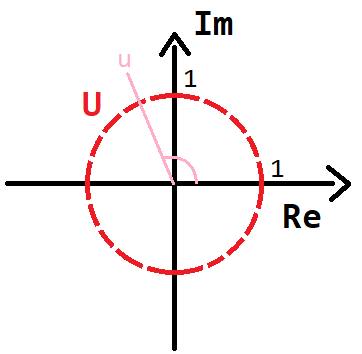
\includegraphics[scale=0.5]{immagini/pianoComplessoUnitari}
	\caption{ Piano complesso con i numeri unitari }
	\label{fig: piano complesso unitari}
\end{figure}

\textbf{Moltiplicazione tra due numeri complessi unitari:} \\
Prendiamo due numeri complessi $ u = cos\theta +j sin\theta $ e $ s = \rho ( cos( Arg(s) ) + j sin ( Arg(s) ) ) $ \\
allora $ s u = \rho ( \cos ( Arg(s) + \theta) + j \sin (Arg(s) + \theta) ) $

Graficamente abbiamo:
\begin{figure}[h]
	\centering
	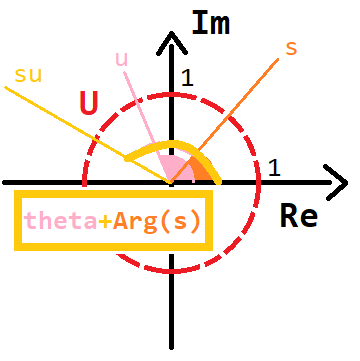
\includegraphics[scale=0.5]{immagini/ComplessiUnitariMoltiplicazioni}
	\caption{ Somma degli argomenti di due numeri complessi unitari }
	\label{fig: complesso unitari moltiplicazioni}
\end{figure}

\subsection*{Potenze dei numeri complessi}
Prendiamo un numero complesso $ s = \rho (cos\theta + j sen\theta) $ \\
la sua potenza ennesima sarà $ s^{n} = \rho^{n} (cos(n\theta) + j sen(n\theta ) ) $ sempre ricordando che $n\theta \in (-\pi , \pi ]$.

\subsection*{Radice nei complessi}

Dato $ s = \rho (cos\theta + j sen\theta) $ vogliamo trovare $ w = r (cos\alpha + j sen \alpha )$ tale che $ w^{n} = s$ , cioè w è la radice n-sima di un numero complesso s. \\
s ha n radici complesse, prendiamo $ w_{k} = r (cos\alpha_{k} + j sen \alpha_{k} ) $ con $r = \sqrt{\rho}$ , $ \alpha_{k} = \frac{\theta}{ n} + k \frac{2 \pi}{n} $ e $ k = 0,1,...,n-1$ \\
allora abbiamo che $ w_{k} = s$. \\

Per $ k = 0$ avremo che $ |w_{0}| = \sqrt[n]{ \rho}  $ e $ Arg(w_{0}) = \frac{1}{n} Arg(s)$.\\

\subsection*{Radici complesse dell'unità}

Definiamo l'unità come $s=1$, è comunque un numero complesso unitario ($ |s| = 1$) e quindi anche lui avrà n radici.\\

\begin{figure}[h]
	\centering
	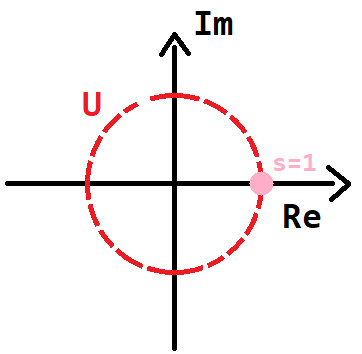
\includegraphics[scale=0.5]{immagini/pianoComplessoUnitari-s}
	\caption{ s=1, numero complesso unitario }
	\label{fig: numero complesso unitario}
\end{figure}


Posso vedere $s=1$ come: $ cos0 + j sen0 $. \\
Qual è quel numero $ w_{k} =  cos\alpha_{k} + j sen \alpha_{k} $ tale che $ w_{k}^{n} = s = 1$? (NB: $ r =1 $ perchè s è unitario cioè il modulo è uguale a 1. NB: dobbiamo trovare $ \alpha_{k}$).\\
$ cos \alpha_{k} $ deve essere uguale a $ cos0 $ e $ sen \alpha_{k} $ deve essere uguale a $ sen0 $. Perciò $\alpha_{k}$ non può essere altro che uguale a $ 0 $ ma anche uguale a tutti i multipli $ 2 \pi$, avrò quindi $ \alpha_{k} = k \frac{ 2 \pi}{n}$ con $ k = 0,1,...,n-1 $.\\

Per $ k = 0$ avremo che $ w_{0} = 1 $ perchè ho proprio $ cos0 + sen0$. \\

Per $ k = 1$ avremo che $ w_{1} = cos(\frac{2 \pi}{n}) + j sen( \frac{2 \pi}{n}) $.\\

\begin{figure}[h]
	\centering
	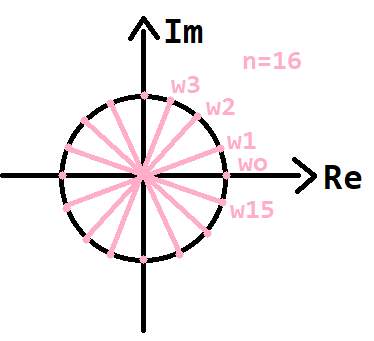
\includegraphics[scale=0.5]{immagini/esempioSUnitario}
	\caption{ n=16, graficamente le radici 16-esime di s=1 }
	\label{fig: esempioRadiciSUNitario}
\end{figure}

Tuttociò è anche dovuto al \textbf{teorema fondamentale dell'algebra} (lo vedremo fra poco) che dice che $ x^{n} = 1$ (con $ x^{n}$ visto come polinomio) avrà n soluzioni complesse. \\

\pagebreak

\section{ Funzioni a variabile complessa }

\subsection*{Def: funzione a variabile complessa}
Definiamo una funzione f a variabile complessa come:
$ f: D(f) \longrightarrow \mathbb{C} $ con $ D(f)\subset \mathbb{C} $ e $ D(f) $ insieme aperto.

\subsection*{Def: insieme aperto}
$ D(f) $ è un insieme aperto $ \Leftrightarrow \forall s_{0} \in D(f) , D(f)\subset \mathbb{C} , \exists $ un disco $ B_{\rho}(s_{0}) \subset D(f)$. \\
$ B_{\rho}(s_{0})$ può essere:\\
- il disco centrato in $ s_{0}$ di raggio $ \rho $\\
- \{ $ s \in \mathbb{C} / |s-s_{0}| < \rho $ \}\\

\textbf{NB: disco = intorno sferico aperto in Analisi 2, aperto = non considero il perimetro}

\begin{figure}[h]
	\centering
	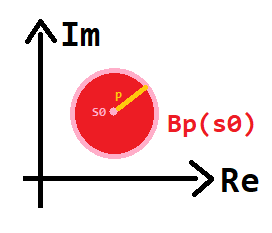
\includegraphics[scale=0.75]{immagini/disco}
	\caption{ Esempio di disco }
	\label{fig: esempioDisco}
\end{figure}


\textbf{NB: In analisi 2 avevamo: } \\
$ B_{\rho}(x_{0}) = $ \{ $ x \in \mathbb{R} / |x-x_{0}| < \rho $ \} $ = ( x_{0}-\rho ... x_{0}+\rho) $

\begin{figure}[h]
	\centering
	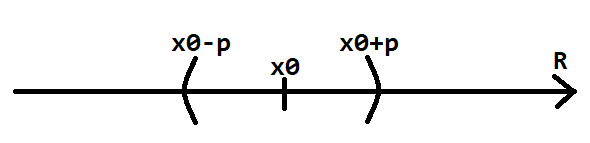
\includegraphics[scale=0.5]{immagini/intornoSfericoAperto}
	\caption{ Intorno sferico aperto }
	\label{fig: intornoSfericoAperto}
\end{figure}

\subsection*{Esempi di insieme aperto}
1) $ D(f) = \mathbb{C} $ cioè tutto il piano complesso.\\
2) $ D(f) = B_{\rho}(s_{0})$ cioè il disco (visto prima).\\

\pagebreak

3) $ D(f) = $ \{ $ s \in \mathbb{C} : \rho_{1} < |s-s_{0}| < \rho_{2} $ \} cioè una corona circolare. \\
\begin{figure}[h]
	\centering
	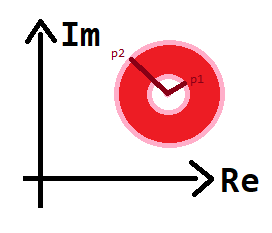
\includegraphics[scale=0.75]{immagini/coronaCircolare}
	\caption{ Esempio di insieme aperto: Corona circolare }
	\label{fig: coronaCircolare}
\end{figure}


4) $ D(f) = $ \{ $ s \in \mathbb{C} : Re(s)> \lambda, \lambda \in \mathbb{R} $ \} cioè il semipiano a destra (Questo è il dominio di definizione della trasformata di Laplace). \\

\begin{figure}[h]
	\centering
	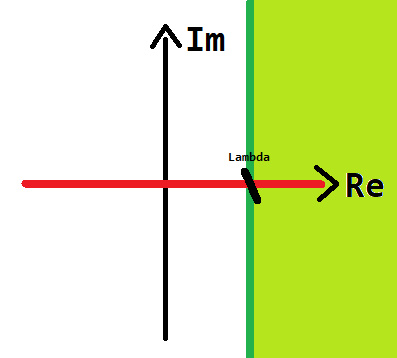
\includegraphics[scale=0.75]{immagini/dominioDefLaplace}
	\caption{ Esempio di insieme aperto: dominio di definizione della trasformata di Laplace }
	\label{fig: dominioDefLaplace}
\end{figure}

5) $D(f) = $ \{ $ s \in \mathbb{C} : Re(s)< \lambda, \lambda \in \mathbb{R} $ \} cioè il semipiano a sinistra. \\ 
6) $D(f) = $ \{ $ s \in \mathbb{C} : Im(s) > Im(j\lambda ), \lambda \in \mathbb{R}, Im(j\lambda ) \in \mathbb{C} $ \} cioè il semipiano superiore. \\

\pagebreak

7) $D(f) = $ \{ $ s \in \mathbb{C} : Im(s) < Im(j\lambda ), \lambda \in \mathbb{R}, Im(j\lambda ) \in \mathbb{C} $ \} cioè il semipiano inferiore (Questo è il dominio di definizione della trasformata di Fourier).\\

\begin{figure}[h]
	\centering
	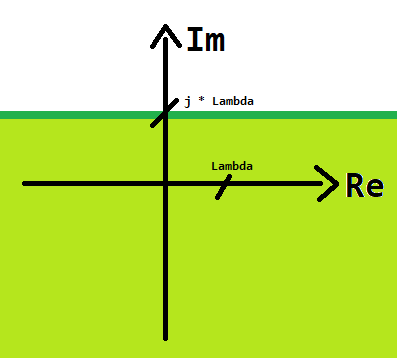
\includegraphics[scale=0.75]{immagini/dominioDefFourier}
	\caption{ Esempio di insieme aperto: dominio di definizione della trasformata di Fourier }
	\label{fig: dominioDefFourier}
\end{figure}

8) $ D(f) = \mathbb{C} \setminus$  \{ $ s_{1},...,s_{n}  $ \}  cioè il piano complesso meno un insieme finito di punti.


\subsection*{Esempi di funzioni a variabili complesse}
1) Funzione identità: $ f(s) = s$ con $ D(f) = \mathbb{C}$.\\
Cioè $ s=x+jy \mapsto s=x+jy $.\\

2) $ f(s) = s^{2}$ con $ D(f) = \mathbb{C}$.\\
Cioè $ s^{2} = (x+jy)^{2} = x^{2}-y^{2} +2jxy $, $ Re(f(s)) = x^{2}-y^{2} $ e $ Im(f(s)) = 2jxy $. \\

3) $ f(s) = s^{n}$ con $ D(f) = \mathbb{C}$.\\
Cioè $ s^{n} = (x+jy)^{n} = \sum_{k=0}^n \binom{n}{k} x^{k} (jy)^{n-k} $ dove ricordo che $ \binom{n}{k} = \frac{n!}{k! (n-k)!} $ il coefficiente binomiale. \\
NB: in coordinate polari diventa \\
Se $ s = \rho (cos\theta + j sen\theta) $ \\
allora $ s^{n} = \rho^{n} (cos(n\theta) + j sen(n\theta ) ) $ \\

4) $ f(s) = \frac{1}{s}$ con $ D(f) = \mathbb{C} \setminus$ \{ 0 \}.\\
Cioè $ \frac{1}{s} = \frac{ \bar{s} }{ |s|^{2}} = \frac{x-jy}{x^{2} + y^{2}} = \frac{ x }{ x^{2} + y^{2} } - j \frac{ y }{ x^{2} + y^{2} } $.\\

5) Funzioni polinomiali:\\
$ P(s) = \sum_{k=0}^n a_{k} s^{k} = a_{n} s^{n} + a_{n-1} s^{n-1} +...+a_{1} s^{1}+a_{0} s^{0} $ con $ a_{k} \in \mathbb{C} $ e $ a_{n} \neq 0$. \\

\textbf{Teorema fondamentale dell'algebra}\\
Ogni polinomio P(s) di grado n ha n radici complesse e si può decomporre in un unico modo:\\
$ P(s) = a_{n} (s- \lambda_{1})^{u_{1}} (s- \lambda_{2})^{u_{2}} ... (s- \lambda_{r})^{u_{r}} $ \\
dove $ \lambda_{1}, \lambda_{2},...,\lambda_{r} $ sono le radici ( cioè $ \forall k $ che va da 1 a r, $ P(\lambda_{k}) = 0$) e $ u_{1},...,u_{r} $ sono le molteplicità.\\

\pagebreak

\textbf{Da questo teorema si evince che:}\\
Tutti i monomi del polinomio sono linearmente indipendenti perchè possiamo vedere lo spazio dei polinomi come uno spazio infinito dimensionale in cui i monomi sono dei vettori. Ogni vettore lo puoi vedere come un vettore della base canonica quindi indipendente dagli altri. Puoi vedere i vettori come coordinate e quindi un monomio del polinomio è una coordinata diversa e a se stante dalle altre. Trovo quindi che $ u_{1}+u_{2}+...+u_{r} = n $.\\
Se prendo $ \lambda_{k} $ in quel punto il polinomio darà zero perchè è una sua radice, cioè $ P(\lambda_{k}) = 0 $. Se derivo il polinomio "gli tolgo una dimensione" ma il monomio non scompare e quindi $ \lambda_{k} $ sarà uno zero anche per la darivata. Avrò che $ P(\lambda_{k}) = P'(\lambda_{k}) = ... = P^{(u_{k}-1)}(\lambda_{k}) = 0 $. \\
Es: $ d(x-2)^3/dx = 3(x-2)^2 $, $ \lambda = 2 $ è radice del polinomio e della sua derivata.\\
Questo però vale fino a $ u_{k}-1 $. Es: $ d 3(x-2)^2/dx = 6(x-2) $ vale ma se derivo ancora $  d 6(x-2)/dx = 6 $ non vale più, cioè $ \lambda_{k} = 2$ non annula questa derivata essendo costante(=6). \\
Vediamo quindi che la derivata di grado $ u_{k} $ cioè uguale alla molteplicità, è la prima derivata non nulla, cioè $ P^{u_{k}}(\lambda_{k}) \neq 0 $.\\

\textbf{OSS1:} nel caso di radici semplici (cioè hanno tutte molteplicità = 1) avrò che:\\
$ P(s) = a_{n} (s- \lambda_{1}) (s- \lambda_{2}) ... (s- \lambda_{r}) $

%TODO: non ho capito questa osservazione
\textbf{OSS2: BOOO???} Se $ a_{k} \in \mathbb{R}$ e $ k=0,...,n $ \\
allora $ \lambda_{k}$ sono tutte radici reali oppure complessi coniugati.\\

\textbf{ES1}\\
$ P_{1}(s) = s^{2} -2s +1 = (s-1)^{2}$\\
Avrò quindi $ \lambda_{1} = 1$ con $ u_{1} = 2$\\
Con $ s=1 $ ho $ P_{1}(1) = 0$.\\
Derivo $ P'_{1}(s) = 2s - 2$.\\
Con $ s=1 $ ho $ P'_{1}(1) = 0$.\\

\textbf{ES2}\\
$ P_{2}(s) = s^{2} +1$\\
Avrò quindi $ \lambda_{1,2} = \pm j$ e $ P_{2}(s) = (s-j)(s+j)$ cioè $ P_{2}( \lambda_{1})=P_{2}( \lambda_{2})=0$\\

6) Funzioni razionali:\\
$ f(s) = \frac{ P(s)}{Q(s)}$ con $ D(f) = \mathbb{C} \setminus$ \{ $ \lambda_{1},..., \lambda_{r}$ \} dove $ \lambda_{k}$ è la radice di $ Q(s)$, cioè $ Q( \lambda_{k})=0$ con $ k=0,...,r$ .\\

\textbf{ES}\\
$ f(s) = \frac{ s^{2}+1}{ s^{2} -1}= \frac{ (s-j)(s+j) }{ (s-1)(s+1)} $ con $ D(f) = \mathbb{C} \setminus$ \{ $ \pm 1$ \}. \\

7) Funzioni come serie di potenze:\\
$ f(s) = \sum_{k=0}^\infty a_{k} (s-s_0)^{k}$ con $ D(f)= \mathbb{C} $. \\
Si associa $r>0$, chiamato \textbf{raggio di convergenza} tale che la serie converge $ \forall s \in Br(s_0) = $ \{ $ s \in \mathbb{C} : |s-s_0| < r$ \} con $ D(f)=Br(s_0)$. La serie non converge per $ s \notin Br(s_0)$.\\

\textbf{ES A): Serie geometrica}\\
$ f(s) = \sum_{k=0}^\infty s^{k} = \sum_{k=0}^\infty (s-0)^{k}$ cioè $s_0= 0$.\\
In questo caso $r=1$ e $ D(f)=B_1(0)=$ \{ $ s \in \mathbb{C} : |s| < 1$ \}.

\pagebreak

\begin{figure}[h]
	\centering
	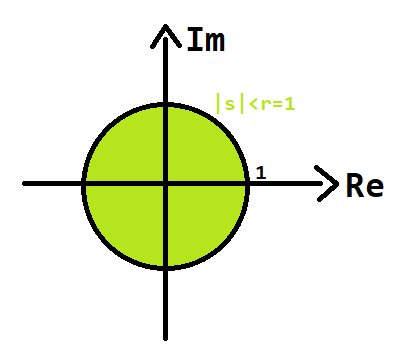
\includegraphics[scale=0.5]{immagini/raggioDiConvergenza}
	\caption{ Graficamente la regione in cui la sommatoria converge }
	\label{fig: raggioDiConvergenza}
\end{figure}

\begin{proof}[Dim:] voglio dimostrare che r=1 è proprio il raggio di convergenza.\\
	Scriviamo $\sum_{k=0}^\infty s^{k} $ come $ \lim_{N \to \infty} \sum_{k=0}^N s^{k} $ per avere questa sommatoria applichiamo un po' di magia di Gregorio (che non fa mai male):\\
	
	$ s^2 -1 = (s-1)(s+1)$\\
	$ s^3 -1 = (s-1)(s^2+s+1 )$\\
	$ s^n -1 = (s-1)(s^{n-1}+ s^{n-2}+...+1)$\\
	Prendiamo quest'ultima equazione, rielaborandola diventa:\\
	$ \frac{ -(s^n -1) }{-(s-1) } = s^{n-1}+ s^{n-2}+...+1$\\
	$ \frac{ 1-s^n }{ 1-s } = s^{n-1}+ s^{n-2}+...+1$\\
	Sostituendo n=N+1 troviamo che:\\
	$ \frac{ 1-s^{N+1} }{ 1-s } = s^N+ s^{N-1}+...+1 = \sum_{k=0}^N s^{k}$\\
	Quindi $ \sum_{k=0}^N s^{k} = \frac{ 1-s^{N+1} }{ 1-s } $
	Ci basta adesso mettere il limite da entrambe le parti:\\
	 $\lim_{N \to \infty} \sum_{k=0}^N s^{k} = \lim_{N \to \infty} \frac{ 1-s^{N+1} }{ 1-s } $, questo ultimo limite dà $ \frac{1}{1-s} $ se $ |s|<1$.\\
	
	Il raggio di convergenza è proprio r=s=1 cioè con $ |r| < 1$ la serie converge (dà un numero finito).\\
	
\end{proof}

\begin{proof}[Dim:] Spiego qui in breve perchè $\lim_{N \to \infty} \frac{ 1-s^{N+1} }{ 1-s } = \frac{1}{1-s} $ se $ |s|<1$.\\
	
	Andiamo per casi:\\
	1) Se $ s>1 $:\\
	Prendiamo come esempio la funzione $ 2^N $.\\
	
	\begin{figure}[h]
		\centering
		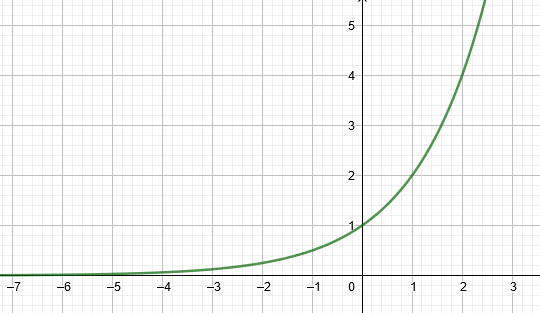
\includegraphics[scale=0.5]{immagini/esp1}
		\caption{ Se s>1 }
		\label{fig: esp1}
	\end{figure}
	
	\pagebreak
	
	Come si può vedere dal grafico il suo limite sarà $ \lim_{N \to \infty} 2^N = \infty $.\\
	Allora in questo caso $ \lim_{N \to \infty} \frac{ 1-s^{N+1} }{ 1-s } = \infty $.\\
	
	2) Se $ 0<s<1 $:\\
	Prendiamo come esempio la funzione $ (\frac{1}{2})^N $.\\
	
	\begin{figure}[h]
		\centering
		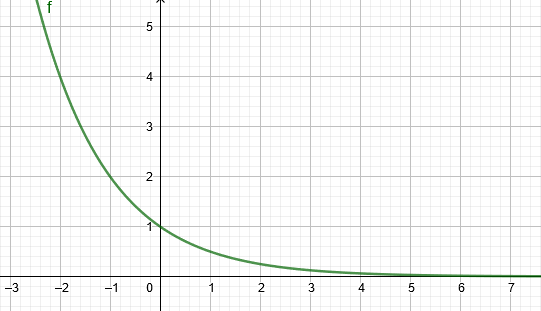
\includegraphics[scale=0.5]{immagini/esp2}
		\caption{ Se 0<s<1 }
		\label{fig: esp2}
	\end{figure}

	Come si può vedere dal grafico il suo limite sarà $ \lim_{N \to \infty} (\frac{1}{2})^N = 0 $.\\
	Allora in questo caso $ \lim_{N \to \infty} \frac{ 1-s^{N+1} }{ 1-s } = \frac{1}{1-s} $.\\
	
	3) Se $ -1<s<0 $:\\
	Prendiamo come esempio la funzione $ (-\frac{1}{2})^N $.\\
	
	\begin{figure}[h]
		\centering
		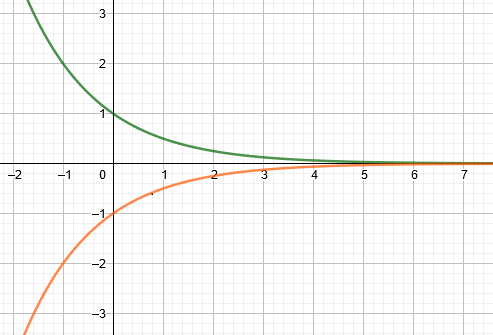
\includegraphics[scale=0.5]{immagini/esp3}
		\caption{ Se -1<s<0 }
		\label{fig: esp3}
	\end{figure}
	
	Come si può vedere dal grafico il suo limite sarà $ \lim_{N \to \infty} (-\frac{1}{2})^N = 0 $.\\
	Allora in questo caso $ \lim_{N \to \infty} \frac{ 1-s^{N+1} }{ 1-s } = \frac{1}{1-s} $.\\
	
	4) Se $ s<-1 $:\\
	Prendiamo come esempio la funzione $ (-2)^N $.\\
	
	\begin{figure}[h]
		\centering
		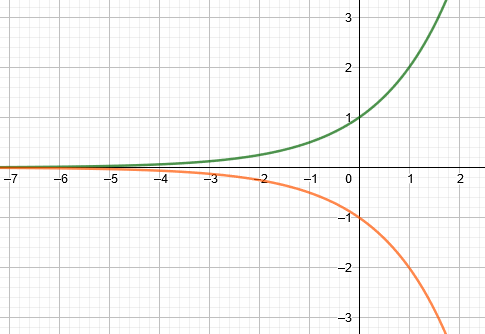
\includegraphics[scale=0.5]{immagini/esp4}
		\caption{ Se s<-1 }
		\label{fig: esp4}
	\end{figure}

	\pagebreak
	
	Come si può vedere dal grafico il suo limite sarà $ \lim_{N \to \infty} (-2)^N = \infty $.\\
	Allora in questo caso $ \lim_{N \to \infty} \frac{ 1-s^{N+1} }{ 1-s } = \infty $.\\
	
	I casi in cui il limite è finito sono 2) e 3), che infatti danno $ |s| < 1$.\\
	
\end{proof}

\textbf{ES B):}\\
Se $ s \longrightarrow -s$ allora $ f(s) = \sum_{k=0}^\infty (-s)^{k} = \sum_{k=0}^\infty (-1)^{k} (s)^k = 1 -s + s^2 - s^3 + s^4 - s^5...$\\
$ = 1 + s^2 + s^4+ ... - s (1 + s^2 + s^4 + ...) = *$\\
NB: $ 1 + s^2 + s^4+ ... = \sum_{k=0}^\infty s^{2k} = \frac{1}{1+s^2}  $\\
Quindi avrò che $* = \frac{1}{1+s^2} - s \frac{1}{1+s^2}$
$ = \frac{1-s}{1+s^2} = \frac{1}{1+s}$\\
Riassumendo ho che $  \sum_{k=0}^\infty (-s)^{k} = \frac{1}{1+s}$.\\
Il raggio di convergenza è come prima $r=1$.\\

\textbf{ES C):}\\
Se $ s \longrightarrow s/a$ allora $ f(s) = \sum_{k=0}^\infty (\frac{s}{a})^k = \frac{1}{1-\frac{s}{a}} = \frac{1}{\frac{a-s}{a}} = \frac{a}{a-s}$\\
Il limite converge con $ |\frac{s}{a}| <1 $.\\
Con raggio di convergenza $ r = |a|$.

%TODO: ci sarebbe un disegno qui ma non lo capisco
\begin{figure}[h]
	\centering
	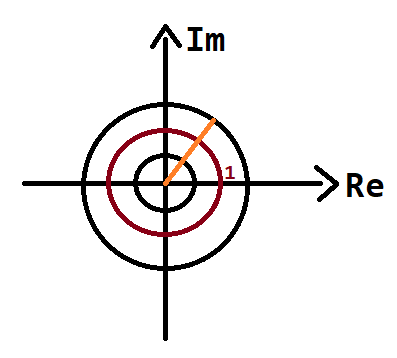
\includegraphics[scale=0.75]{immagini/raggioDiConv2}
	\caption{ Graficamente la regione in cui la sommatoria converge }
	\label{fig: raggioDiConvergenza}
\end{figure}

\pagebreak

\textbf{Prima di andare avanti ripassiamo Taylor e Taylor-Mc Laurin}\\
Data una funzione sufficientemente regolare $ f(x):\mathbb{D} \longrightarrow \mathbb{R} $ con $ \mathbb{D} \subset \mathbb{R} $, è sempre possibile approssimarla in un intorno di un dato punto $ x_0 \in \mathbb{D} $, con polinomi g(x) di grado n. Perchè allora si studiano gli sviluppi di Taylor? Il motivo è che, tra tutti i polinomi di grado n, quello di Taylor è quello che meglio stima la funzione di partenza f in un intorno di $ x_0 $.\\
Possiamo scrivere la serie di Taylor come:\\
 $ f(x) = f(x_0) + \frac{ f'(x_0)}{1!} (x-x_0) + \frac{ f''(x_0)}{2!} (x-x_0)^2 +... = \sum_{n=0}^\infty \frac{ f^{(n)}(x_0) }{n!} (x-x_0)^n$\\
Con sviluppo di Taylor-McLaurin si intende uno sviluppo di Taylor con centro $x_0=0$.
In generale avremo quindi che lo sviluppo di Taylor-McLaurin è:\\
$ f(x) = f(0) + \frac{ f'(0)}{1!} x + \frac{ f''(0)}{2!} x^2+... + \frac{ f^{n}(0)}{n!} x^n+ o(x^n)$ \\

\textbf{ES D): Serie di potenze: funzione esponenziale}\\
$ f(s) = e^{s} = \sum_{k=0}^\infty \frac{s^{k}}{k!} = 1 +s + \frac{s^2}{2} + \frac{s^3}{3!} + \frac{s^4}{4!}+... $.\\
Il raggio di convergenza è $ r = +\infty$ e $ D(f)= \mathbb{C}$.\\

\begin{proof}[Dim:] Dimostriamo che $ e^{s} $ è proprio $\sum_{k=0}^\infty \frac{s^{k}}{k!} $\\ 
	Avendo appena visto la serie di Taylor-McLaurin la dimostrazione è facile. Infatti lo sviluppo in serie di $ e^{s} $ è proprio:\\
	$ e^{x} = e^0 + e^0 x + e^0 \frac{x^2}{2} + e^0 \frac{x^3}{3!} + e^0 \frac{x^4}{4!} +... $ \\
	$ = 1 + x + \frac{x^2}{2} + \frac{x^3}{3!} + \frac{x^4}{4!}+... = \sum_{n=0}^\infty \frac{x^{n}}{n!}$ 
\end{proof}


\textbf{ES E): Funzioni trigonometriche viste come serie}\\
Possiamo scrivere la funzione coseno usando Mc Laurin come:\\
$ g(s) = cos(s) = cos(0) + cos'(0)s + \frac{ cos''(0)}{2!} x^2 + \frac{ cos'''(0)}{3!} x^3 + \frac{ cos''''(0)}{4!} x^4 + ... $\\

Svolgiamo i calcoli: $ cos(0) = 1$ , $ cos'(0)s = -sen(0) = 0 $, $\frac{ cos''(0)}{2!} x^2 = - \frac{ cos(0)}{2!} x^2 = - \frac{ x^2}{2!}$, $ \frac{ cos'''(0)}{3!} x^3 = 0 $ e $ \frac{ cos''''(0)}{4!} x^4 = \frac{ x^4}{4!} $.

Quindi avrò $ g(s) = cos(s) = 1 + 0 - \frac{s^2}{2!} + 0 + \frac{s^4}{4!} + 0 -... $\\


Da notare come i segni si continuino ad alternare, questo è dovuto alle derivate del coseno e del seno:\\
$ (cos(s))' = - sen(s)$\\
$ (sen(s))' = cos(s)$\\

Riscrivendolo avrò che $  g(s) = cos(s) = 1 - \frac{s^2}{2!} + \frac{s^4}{4!} -...$, questo si può scrivere anche come $ \sum_{k=0}^\infty (-1)^k \dfrac{s^{2k}}{(2k)!}$. \\

Possiamo vedere anche il seno come serie:\\
$ g(s)=sen(s)= \sum_{k=0}^\infty (-1)^k \dfrac{s^{2k+1}}{(2k+1)!} = s - \frac{s^3}{3!}+\frac{s^5}{5!}-...$

\pagebreak

\textbf{COMANDO MATLAB:}\\

\begin{figure}[h]
	\centering
	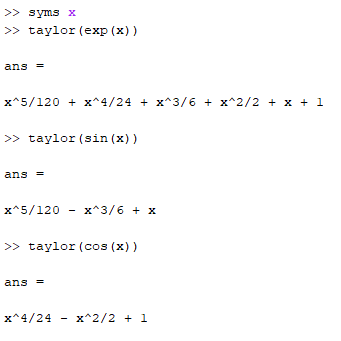
\includegraphics{immagini/comando1}
	\caption{ Il comando syms crea variabili, in questo caso x }
	\label{fig: Primo comando Matlab}
\end{figure}

\textbf{Rappresentazione esponenziale di un numero complesso}\\
Mettiamo nell'equazione $ e^s = \sum_{k=0}^\infty \frac{s^k}{k!}$, $s=jw$ un numero complesso immaginario puro.\\
Verrà fuori che $ e^{jw} = 1 + jw + \frac{(jw)^2}{2!}+ \frac{(jw)^3}{3!}+ \frac{(jw)^4}{4!}+... $.\\
Svolgiamo i calcoli: $ j^0 = 1$ , $ j^1 = j $ ,$j^2=-1 $, $ j^3=-j $, $j^4 = -jj= 1$ e così via...\\
Come si può vedere c'è un pattern che continua a ripetersi 1,j,-1,-j. Vogliamo avere le coppie (1,-1) da una parte e (j,-j) da un'altra. Raggruppiamo tutti i fattori senza j a sinistra e isoliamo j (puoi anche vedere che tutti gli esponenti pari vanno a sinistra e tutti quelli dispari vanno fra parentesi a destra), ci verrà fuori che: \\
$ e^{jw} = 1 +jw-\frac{(w)^2}{2!} -j\frac{(w)^3}{3!}+\frac{(w)^4}{4!}+j\frac{(w)^5}{5!}-... $\\
$ = 1-\frac{(w)^2}{2!}+\frac{(jw)^4}{4!}-\frac{(jw)^6}{6!}+...+j(w - \frac{w^3}{3!}+\frac{w^5}{5!}-...)$\\
Tutto quello a sinistra è $ cos(w) $ mentre tutto quello nella parentesi è $ sen(w)$, avrò quindi che:\\
$ e^{jw} = cosw +jsenw$.\\
NB: $ Re(e^{jw}) = cosw $ e $ Im(e^{jw}) = senw$.\\

\begin{figure}[h]
	\centering
	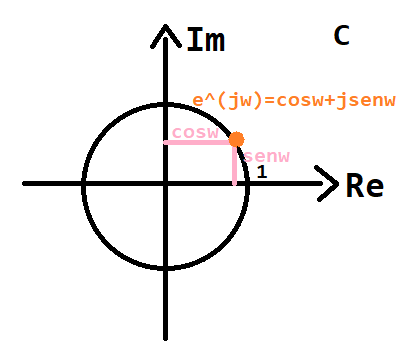
\includegraphics[scale=0.5]{immagini/rappEsp}
	\caption{ Rappresentazione grafica }
	\label{fig: rappEsp}
\end{figure}

\textbf{Nel caso generale:}\\
$ s = \rho ( cos \theta + sen \theta ) = \rho e^{j \theta} $.\\

\textbf{Casi particolari}\\
1) Se $ w = \pi $ allora $ e^{j \pi} = cos( \pi) + j sen(\pi) = -1$. Cioè $ e^{j \pi} +1=0 $ che è l'\textbf{identità di Eurelo}.\\
2) Se $ w = \pi/2 $ allora $ e^{j\frac{\pi}{2}} = cos( \frac{\pi}{2}) + j sen(\frac{\pi}{2}) = j$.\\
3) Se $ w = -w $ allora $ e^{-jw} = cos( -w) + j sen(-w) = cosw-jsenw $, cioè è il coniugato complesso. Infatti $ e^{jw} e^{-jw} = e^{0} = 1 $.\\
4) Sommiamo fra loro $e^{jw}$ e $e^{-jw}$ verrà fuori che:\\
$ e^{jw} + e^{-jw} = 2 cosw $ allora $ cosw = \frac{e^{jw} + e^{-jw}}{2} $.\\
5) Se invece li sottraiamo vediamo che:\\
$ e^{jw} - e^{-jw} = cosw+jsenw-(cosw-senw)=2jsenw $ allora $ senw = \frac{e^{jw} - e^{-jw}}{2j} $.\\


\textbf{Conviene vedere tutte le funzioni come complesse visto che avrò a che fare con equazioni differenziali.}



















